\documentclass{standalone}
\usepackage{tikz}
\usetikzlibrary{patterns, positioning}
\usepackage[sfdefault]{ClearSans} %% option 'sfdefault' activates Clear Sans as the default text font
\usepackage[T1]{fontenc}

\begin{document}
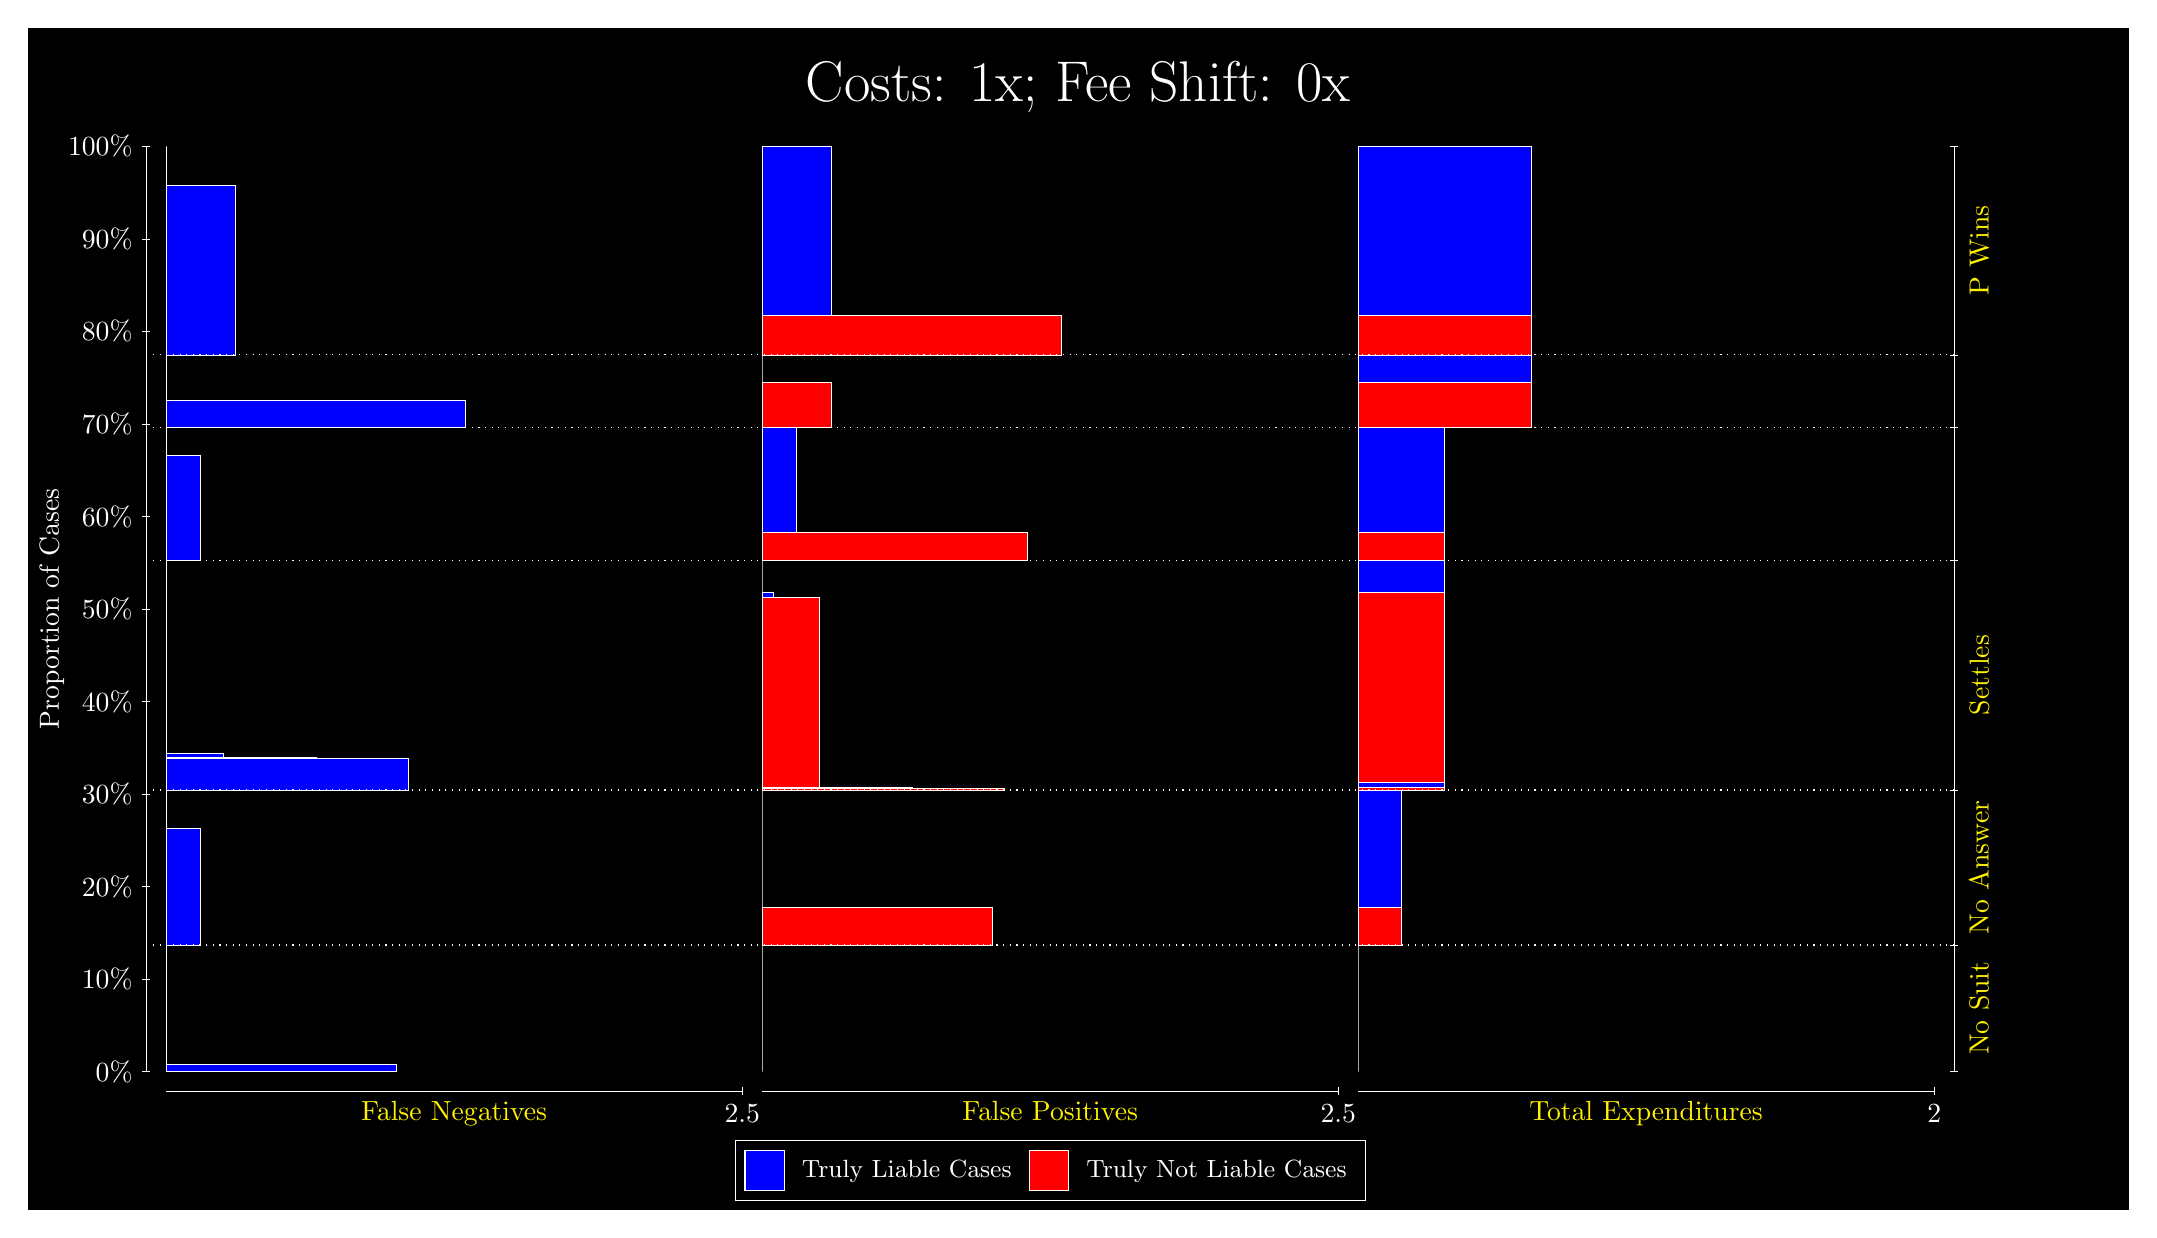
\begin{tikzpicture}
\draw[fill=black] (0,0) rectangle (26.667,15);
\draw[text=white] (0,13.5) rectangle (26.667,15) node[midway] {\huge Costs: 1x; Fee Shift: 0x};
\draw[white, very thin] (1.5,1.75) -- (1.5,13.5);
\node[rotate=90, text=white, anchor=center] at (0.3, 7.625) {Proportion of Cases};
\draw[white, very thin] (1.45,1.75) -- (1.55,1.75);
\node[text=white, anchor=east] at (1.45, 1.75) {0\%};
\draw[white, very thin] (1.45,2.925) -- (1.55,2.925);
\node[text=white, anchor=east] at (1.45, 2.925) {10\%};
\draw[white, very thin] (1.45,4.1) -- (1.55,4.1);
\node[text=white, anchor=east] at (1.45, 4.1) {20\%};
\draw[white, very thin] (1.45,5.275) -- (1.55,5.275);
\node[text=white, anchor=east] at (1.45, 5.275) {30\%};
\draw[white, very thin] (1.45,6.45) -- (1.55,6.45);
\node[text=white, anchor=east] at (1.45, 6.45) {40\%};
\draw[white, very thin] (1.45,7.625) -- (1.55,7.625);
\node[text=white, anchor=east] at (1.45, 7.625) {50\%};
\draw[white, very thin] (1.45,8.8) -- (1.55,8.8);
\node[text=white, anchor=east] at (1.45, 8.8) {60\%};
\draw[white, very thin] (1.45,9.975) -- (1.55,9.975);
\node[text=white, anchor=east] at (1.45, 9.975) {70\%};
\draw[white, very thin] (1.45,11.15) -- (1.55,11.15);
\node[text=white, anchor=east] at (1.45, 11.15) {80\%};
\draw[white, very thin] (1.45,12.325) -- (1.55,12.325);
\node[text=white, anchor=east] at (1.45, 12.325) {90\%};
\draw[white, very thin] (1.45,13.5) -- (1.55,13.5);
\node[text=white, anchor=east] at (1.45, 13.5) {100\%};

\draw[white, very thin] (24.457,1.75) -- (24.457,13.5);
\draw[white, very thin] (24.407,1.75) -- (24.507,1.75);
\node[anchor=west] at (24.407, 1.75) {};
\draw[white, very thin] (24.407,3.3575) -- (24.507,3.3575);
\node[anchor=west] at (24.407, 3.3575) {};
\draw[white, very thin] (24.407,5.3258) -- (24.507,5.3258);
\node[anchor=west] at (24.407, 5.3258) {};
\draw[white, very thin] (24.407,8.2451) -- (24.507,8.2451);
\node[anchor=west] at (24.407, 8.2451) {};
\draw[white, very thin] (24.407,9.9297) -- (24.507,9.9297);
\node[anchor=west] at (24.407, 9.9297) {};
\draw[white, very thin] (24.407,10.852) -- (24.507,10.852);
\node[anchor=west] at (24.407, 10.852) {};
\draw[white, very thin] (24.407,13.5) -- (24.507,13.5);
\node[anchor=west] at (24.407, 13.5) {};

\draw[white, very thin, fill=blue] (1.75,1.75) rectangle (4.6775,1.8442);
\draw[white, very thin, fill=red] (1.75,1.8442) rectangle (1.75,3.3575);
\draw[white, very thin, fill=blue] (1.75,3.3575) rectangle (2.1891,4.8417);
\draw[white, very thin, fill=red] (1.75,4.8417) rectangle (1.75,5.3258);
\draw[white, very thin, fill=blue] (1.75,5.3258) rectangle (4.8239,5.7346);
\draw[white, very thin, fill=blue] (1.75,5.7346) rectangle (3.6529,5.7379);
\draw[white, very thin, fill=blue] (1.75,5.7379) rectangle (2.4819,5.7957);
\draw[white, very thin, fill=red] (1.75,5.7957) rectangle (1.75,8.2451);
\draw[white, very thin, fill=blue] (1.75,8.2451) rectangle (2.1891,9.5776);
\draw[white, very thin, fill=red] (1.75,9.5776) rectangle (1.75,9.9297);
\draw[white, very thin, fill=blue] (1.75,9.9297) rectangle (5.5558,10.275);
\draw[white, very thin, fill=red] (1.75,10.275) rectangle (1.75,10.852);
\draw[white, very thin, fill=blue] (1.75,10.852) rectangle (2.6283,13.001);
\draw[white, very thin, fill=red] (1.75,13.001) rectangle (1.75,13.5);
\draw[white, very thin, fill=red] (9.3189,1.75) rectangle (9.3189,3.2633);
\draw[white, very thin, fill=blue] (9.3189,3.2633) rectangle (9.3189,3.3575);
\draw[white, very thin, fill=red] (9.3189,3.3575) rectangle (12.246,3.8416);
\draw[white, very thin, fill=blue] (9.3189,3.8416) rectangle (9.3189,5.3258);
\draw[white, very thin, fill=red] (9.3189,5.3258) rectangle (12.393,5.3411);
\draw[white, very thin, fill=red] (9.3189,5.3411) rectangle (11.222,5.3562);
\draw[white, very thin, fill=red] (9.3189,5.3562) rectangle (10.051,7.7752);
\draw[white, very thin, fill=blue] (9.3189,7.7752) rectangle (9.4652,7.833);
\draw[white, very thin, fill=blue] (9.3189,7.833) rectangle (9.3189,8.2451);
\draw[white, very thin, fill=red] (9.3189,8.2451) rectangle (12.686,8.5971);
\draw[white, very thin, fill=blue] (9.3189,8.5971) rectangle (9.758,9.9297);
\draw[white, very thin, fill=red] (9.3189,9.9297) rectangle (10.197,10.507);
\draw[white, very thin, fill=blue] (9.3189,10.507) rectangle (9.3189,10.852);
\draw[white, very thin, fill=red] (9.3189,10.852) rectangle (13.125,11.351);
\draw[white, very thin, fill=blue] (9.3189,11.351) rectangle (10.197,13.5);
\draw[white, very thin, fill=red] (16.888,1.75) rectangle (16.888,3.2633);
\draw[white, very thin, fill=blue] (16.888,3.2633) rectangle (16.888,3.3575);
\draw[white, very thin, fill=red] (16.888,3.3575) rectangle (17.437,3.8416);
\draw[white, very thin, fill=blue] (16.888,3.8416) rectangle (17.437,5.3258);
\draw[white, very thin, fill=red] (16.888,5.3258) rectangle (17.986,5.3562);
\draw[white, very thin, fill=blue] (16.888,5.3562) rectangle (17.986,5.4173);
\draw[white, very thin, fill=red] (16.888,5.4173) rectangle (17.986,7.8363);
\draw[white, very thin, fill=blue] (16.888,7.8363) rectangle (17.986,8.2451);
\draw[white, very thin, fill=red] (16.888,8.2451) rectangle (17.986,8.5971);
\draw[white, very thin, fill=blue] (16.888,8.5971) rectangle (17.986,9.9297);
\draw[white, very thin, fill=red] (16.888,9.9297) rectangle (19.083,10.507);
\draw[white, very thin, fill=blue] (16.888,10.507) rectangle (19.083,10.852);
\draw[white, very thin, fill=red] (16.888,10.852) rectangle (19.083,11.351);
\draw[white, very thin, fill=blue] (16.888,11.351) rectangle (19.083,13.5);
\draw[white, dotted] (1.5,3.3575) -- (24.457,3.3575);
\draw[white, dotted] (1.5,5.3258) -- (24.457,5.3258);
\draw[white, dotted] (1.5,8.2451) -- (24.457,8.2451);
\draw[white, dotted] (1.5,9.9297) -- (24.457,9.9297);
\draw[white, dotted] (1.5,10.852) -- (24.457,10.852);
\draw[white, very thin] (1.75,1.5) -- (9.0689,1.5);
\node[text=yellow, anchor=north] at (5.4094, 1.5) {False Negatives};
\draw[white, very thin] (9.0689,1.45) -- (9.0689,1.55);
\node[text=white, anchor=north] at (9.0689, 1.45) {2.5};

\draw[white, very thin] (9.3189,1.5) -- (16.638,1.5);
\node[text=yellow, anchor=north] at (12.978, 1.5) {False Positives};
\draw[white, very thin] (16.638,1.45) -- (16.638,1.55);
\node[text=white, anchor=north] at (16.638, 1.45) {2.5};

\draw[white, very thin] (16.888,1.5) -- (24.207,1.5);
\node[text=yellow, anchor=north] at (20.547, 1.5) {Total Expenditures};
\draw[white, very thin] (24.207,1.45) -- (24.207,1.55);
\node[text=white, anchor=north] at (24.207, 1.45) {2};

\node[text=yellow, centered, rotate=90] at (24.777, 2.5537) {No Suit};
\node[text=yellow, centered, rotate=90] at (24.777, 4.3417) {No Answer};
\node[text=yellow, centered, rotate=90] at (24.777, 6.7855) {Settles};


\node[text=yellow, centered, rotate=90] at (24.777, 12.176) {P Wins};

\draw (12.978300999999998,1.5) node[draw=none] (baseCoordinate) {};
\begin{scope}[align=center]
        \matrix[scale=0.5, draw=white, below=0.5cm of baseCoordinate, nodes={draw}, column sep=0.1cm]{
            \node[rectangle, draw, minimum width=0.5cm, minimum height=0.5cm, fill=blue] {}; &
            \node[draw=none, font=\small, text=white] (B) {Truly Liable Cases}; &
            \node[rectangle, draw, minimum width=0.5cm, minimum height=0.5cm, fill=red] {}; &
            \node[draw=none, font=\small, text=white] (B) {Truly Not Liable Cases}; \\
            };
\end{scope}

\end{tikzpicture}
\end{document}